\chapter{Gestão do projeto}

A gestão do projeto é fundamental para garantir que o desenvolvimento da solução ocorra de forma organizada, controlada e alinhada aos objetivos estabelecidos. De acordo com a Escola Nacional de Administração Pública (ENAP, 2014), o gerenciamento de projetos consiste na aplicação de conhecimentos, habilidades, ferramentas e técnicas às atividades do projeto, envolvendo planejamento, execução e controle para atender aos requisitos definidos. Destaca-se que projetos são temporários e voltados à entrega de resultados únicos (ENAP, 2014), o que se aplica ao EIGAM, já que o sistema proposto possui escopo, prazo e entregas previamente definidos.

Para apoiar essa organização, foram utilizadas ferramentas digitais, listadas no Quadro~\ref{frame:recursos}, que auxiliaram o planejamento, o acompanhamento das tarefas e o desenvolvimento do sistema. Um quadro de tarefas \textit{on-line} foi empregado na visualização e no controle das atividades de concepção, enquanto um serviço de hospedagem de repositórios Git foi utilizado para armazenamento e versionamento do código-fonte, favorecendo a colaboração entre os integrantes da equipe.

\section{Gerenciamento do projeto}

Para o gerenciamento do projeto, optou-se pela utilização de práticas ágeis, com destaque para o \textit{framework} Scrum, por sua flexibilidade e adequação ao desenvolvimento incremental de \textit{software}. Segundo o Guia do Scrum, essa abordagem permite organizar o trabalho em ciclos curtos, com entregas contínuas, revisão frequente e adaptação ao longo do processo, o que favorece maior controle e acompanhamento do desenvolvimento (SCHWABER; SUTHERLAND, 2020).

Na fase de desenvolvimento, o \textit{backlog} foi versionado no próprio repositório, organizado como um quadro Kanban, com as listas \textit{Backlog}, \textit{Sprint} Atual, Em andamento, Revisão e Concluído. Essa escolha permitiu consultar e atualizar os cartões no mesmo repositório do código, inclusive pelo assistente de programação utilizado pela equipe. Cada cartão trazia critérios de aceitação verificáveis, e os cartões foram organizados em 15 \textit{sprints} temáticas, ordenadas por dependência técnica: fundação, infraestrutura, esqueleto ponta a ponta, cadastro e autenticação, núcleo financeiro, análise financeira, conversa com IA, notificações, LGPD e qualidade, cobrança, produção, painel de operação, painel do titular, conversa financeira e MCP do titular.

A terceira \textit{sprint} fechou o ciclo completo de uma mensagem, do WhatsApp ao \textit{broker}, ao serviço de conversa e de volta ao WhatsApp, antes de qualquer funcionalidade. A integração com o provedor do WhatsApp era o maior risco técnico do projeto, e validá-la cedo evitou que as demais funcionalidades fossem construídas sobre uma premissa não comprovada. A definição de pronto exigia todos os critérios do cartão cumpridos, testes aprovados sem queda de cobertura, documentação de arquitetura atualizada quando um contrato mudava e, para mudanças de \textit{prompt} ou modelo, a execução dos conjuntos de referência.

O serviço de hospedagem de repositórios deu suporte ao versionamento do sistema, distribuído em dezenove repositórios (um monorrepositório que agrega os outros dezoito como submódulos), e ao registro das alterações realizadas. As mensagens de \textit{commit} seguiram o padrão Conventional Commits, e a integração contínua executou, a cada alteração, análise estática, verificação de tipos, testes com cobertura mínima e \textit{build}, além de publicar a imagem do serviço quando a alteração era incorporada à \textit{branch} principal. As decisões difíceis de reverter foram documentadas em registros de decisão de arquitetura (\textit{Architecture Decision Records}, ADRs), que serviram de memória técnica do projeto. Dessa forma, a combinação entre Scrum, \textit{backlog} versionado, controle de versões e integração contínua tornou o desenvolvimento mais rastreável, colaborativo e alinhado às entregas previstas.

\section{Detalhamento das atividades}

As atividades do projeto foram agrupadas por fase, abrangendo desde a concepção do produto até a entrega final. O Quadro~\ref{frame:atividades} apresenta o conjunto de atividades realizadas: as de 1 a 18 correspondem à fase de concepção, apresentada na Figura~\ref{fig:cronograma}, e as de 19 a 27, à fase de desenvolvimento, cujo cronograma executado é apresentado por componente, e não por atividade, na Figura~\ref{fig:cronograma_dev}.

\begin{table}[H]
\centering
\caption{Detalhamento das atividades}
\label{frame:atividades}
\begin{tabular}{|c|L{10cm}|}
\hline
\textbf{Número} & \textbf{Atividade} \\ \hline
1 & Identificação da oportunidade de negócios \\ \hline
2 & Análise de mercado \\ \hline
3 & Definição do produto \\ \hline
4 & Planejamento e estruturação do projeto \\ \hline
5 & Definição do público-alvo \\ \hline
6 & Elaboração das personas de negócio \\ \hline
7 & Criação do Canvas de negócio \\ \hline
8 & Análise de viabilidade do projeto \\ \hline
9 & Pesquisa por meio de questionário \\ \hline
10 & Definição do preço de venda \\ \hline
11 & Mapeamento de recursos \\ \hline
12 & Elaboração do cronograma do projeto \\ \hline
13 & Elicitação de requisitos \\ \hline
14 & Modelagem do sistema \\ \hline
15 & Prototipagem de telas \\ \hline
16 & Modelagem do banco de dados \\ \hline
17 & Elaboração da proposta de desenvolvimento \\ \hline
18 & Definição de padrões de projeto \\ \hline
19 & Provisionamento da infraestrutura e da integração contínua \\ \hline
20 & Implementação do ciclo ponta a ponta da mensagem \\ \hline
21 & Implementação do cadastro, da autenticação e da cobrança \\ \hline
22 & Integração com o Open Finance e análise financeira \\ \hline
23 & Implementação da camada conversacional e de IA \\ \hline
24 & Implementação dos direitos do titular, dos avisos e dos resumos \\ \hline
25 & Implementação dos painéis \textit{web} \\ \hline
26 & Testes, validação de qualidade e teste de carga \\ \hline
27 & Elaboração dos resultados e finalização do trabalho \\ \hline
\end{tabular}

\authorssource
\end{table}

\section{Detalhamento dos recursos}

As informações contidas no Quadro~\ref{frame:recursos} permitem identificar, de forma organizada, os recursos disponíveis e os recursos demandados pelo projeto, envolvendo equipe, equipamentos, \textit{softwares} e infraestrutura fundamentais para sua execução.

\begin{table}[H]
\centering
\caption{Detalhamento dos recursos}
\label{frame:recursos}
\begin{tabular}{|l|L{7cm}|l|}
\hline
\textbf{Tipo} & \textbf{Descrição} & \textbf{Situação} \\ \hline
\multirow{3}{*}{Equipe} & Marco Antônio Lonardon Júnior & Disponível \\ \cline{2-3}
 & Matheus Lima Bonadio & Disponível \\ \cline{2-3}
 & Vitor Nascimento Moreira & Disponível \\ \hline
\multirow{2}{*}{Equipamentos} & MacBook com processador M2 & Disponível \\ \cline{2-3}
 & Acesso à internet & Disponível \\ \hline
\multirow{8}{*}{\textit{Softwares}} & Trello & Disponível \\ \cline{2-3}
 & Google Forms & Disponível \\ \cline{2-3}
 & Figma & Disponível \\ \cline{2-3}
 & Visual Studio Code & Disponível \\ \cline{2-3}
 & Claude Code & Disponível \\ \cline{2-3}
 & GitHub e GitHub Actions & Disponível \\ \cline{2-3}
 & Docker & Disponível \\ \cline{2-3}
 & Terraform & Disponível \\ \hline
\multirow{2}{*}{Infraestrutura} & Servidor Hetzner Cloud CX33 & Contratado \\ \cline{2-3}
 & Domínio \texttt{eigam.com.br} e Cloudflare & Contratado \\ \hline
\multirow{6}{*}{Serviços} & MongoDB Atlas (banco de dados documental gerenciado) & Contratado \\ \cline{2-3}
 & Pluggy (agregador de Open Finance) & Contratado \\ \cline{2-3}
 & OpenAI (provedor do modelo de linguagem) & Contratado \\ \cline{2-3}
 & Stripe (provedor de pagamentos) & Contratado \\ \cline{2-3}
 & WhatsApp Business Platform & Contratado \\ \cline{2-3}
 & Telegram Bot API & Disponível \\ \hline
\end{tabular}

\authorssource
\end{table}

\section{Cronograma do projeto}

O cronograma apresentado na Figura~\ref{fig:cronograma} detalha as tarefas da fase de concepção, indicando quem foi responsável por cada tarefa e quanto tempo foi necessário para sua realização.

\begin{figure}[H]
    \centering
    \caption{Cronograma da fase de concepção}
    \label{fig:cronograma}
    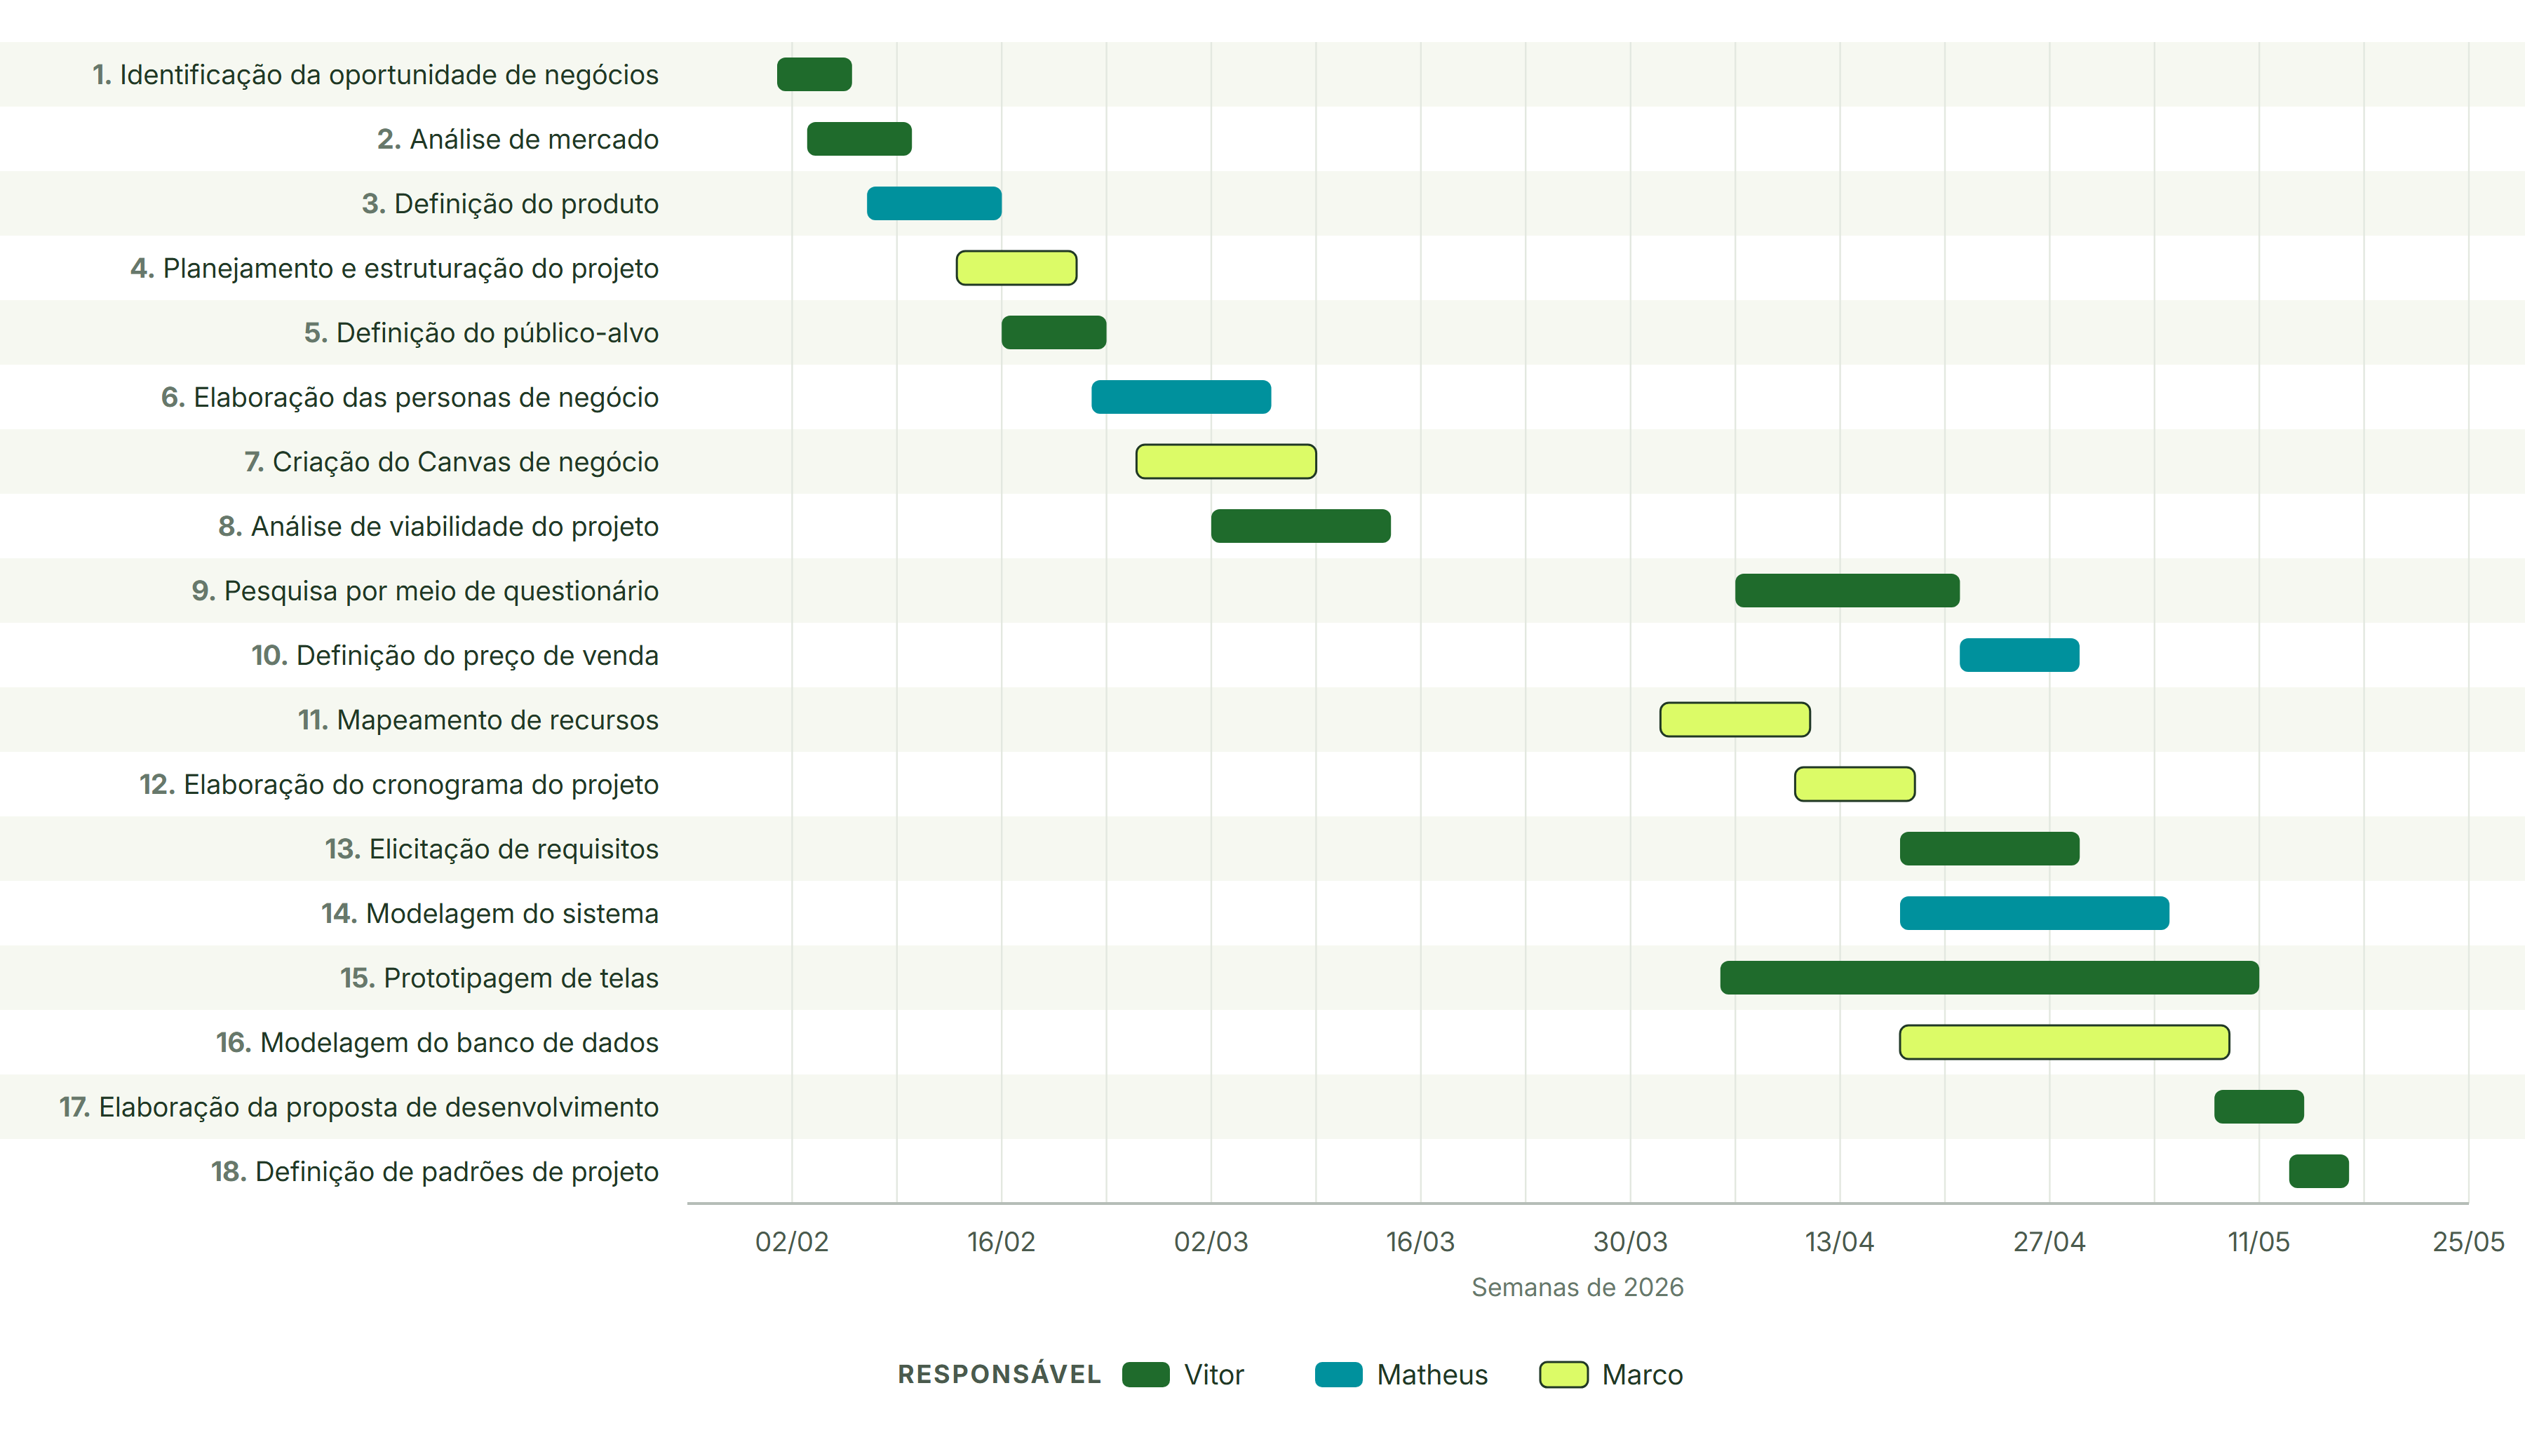
\includegraphics[width=1\textwidth]{images/cronograma.png}
    \authorssource
\end{figure}

A Figura~\ref{fig:cronograma_dev} apresenta o cronograma da fase de desenvolvimento, construído a partir do histórico dos repositórios: cada barra vai do primeiro ao último \textit{commit} do componente, e os marcos correspondem a decisões e validações registradas nos ADRs e nos relatórios técnicos. Os serviços centrais foram criados juntos, na primeira semana, porque o ciclo ponta a ponta da mensagem foi validado primeiro. Os painéis \textit{web} foram construídos no fim da fase, para a operação do sistema e para a consulta de períodos longos pelo titular, e o servidor MCP foi o último componente incorporado, seguido da inclusão do período de teste no catálogo de planos e da integração de metas, alertas e projeção, que encerrou a fase. Ao todo, foram mais de 3.100 \textit{commits}, com pico de atividade na semana em que foram construídos os painéis e os resumos periódicos.

\begin{figure}[H]
    \centering
    \caption{Cronograma executado na fase de desenvolvimento}
    \label{fig:cronograma_dev}
    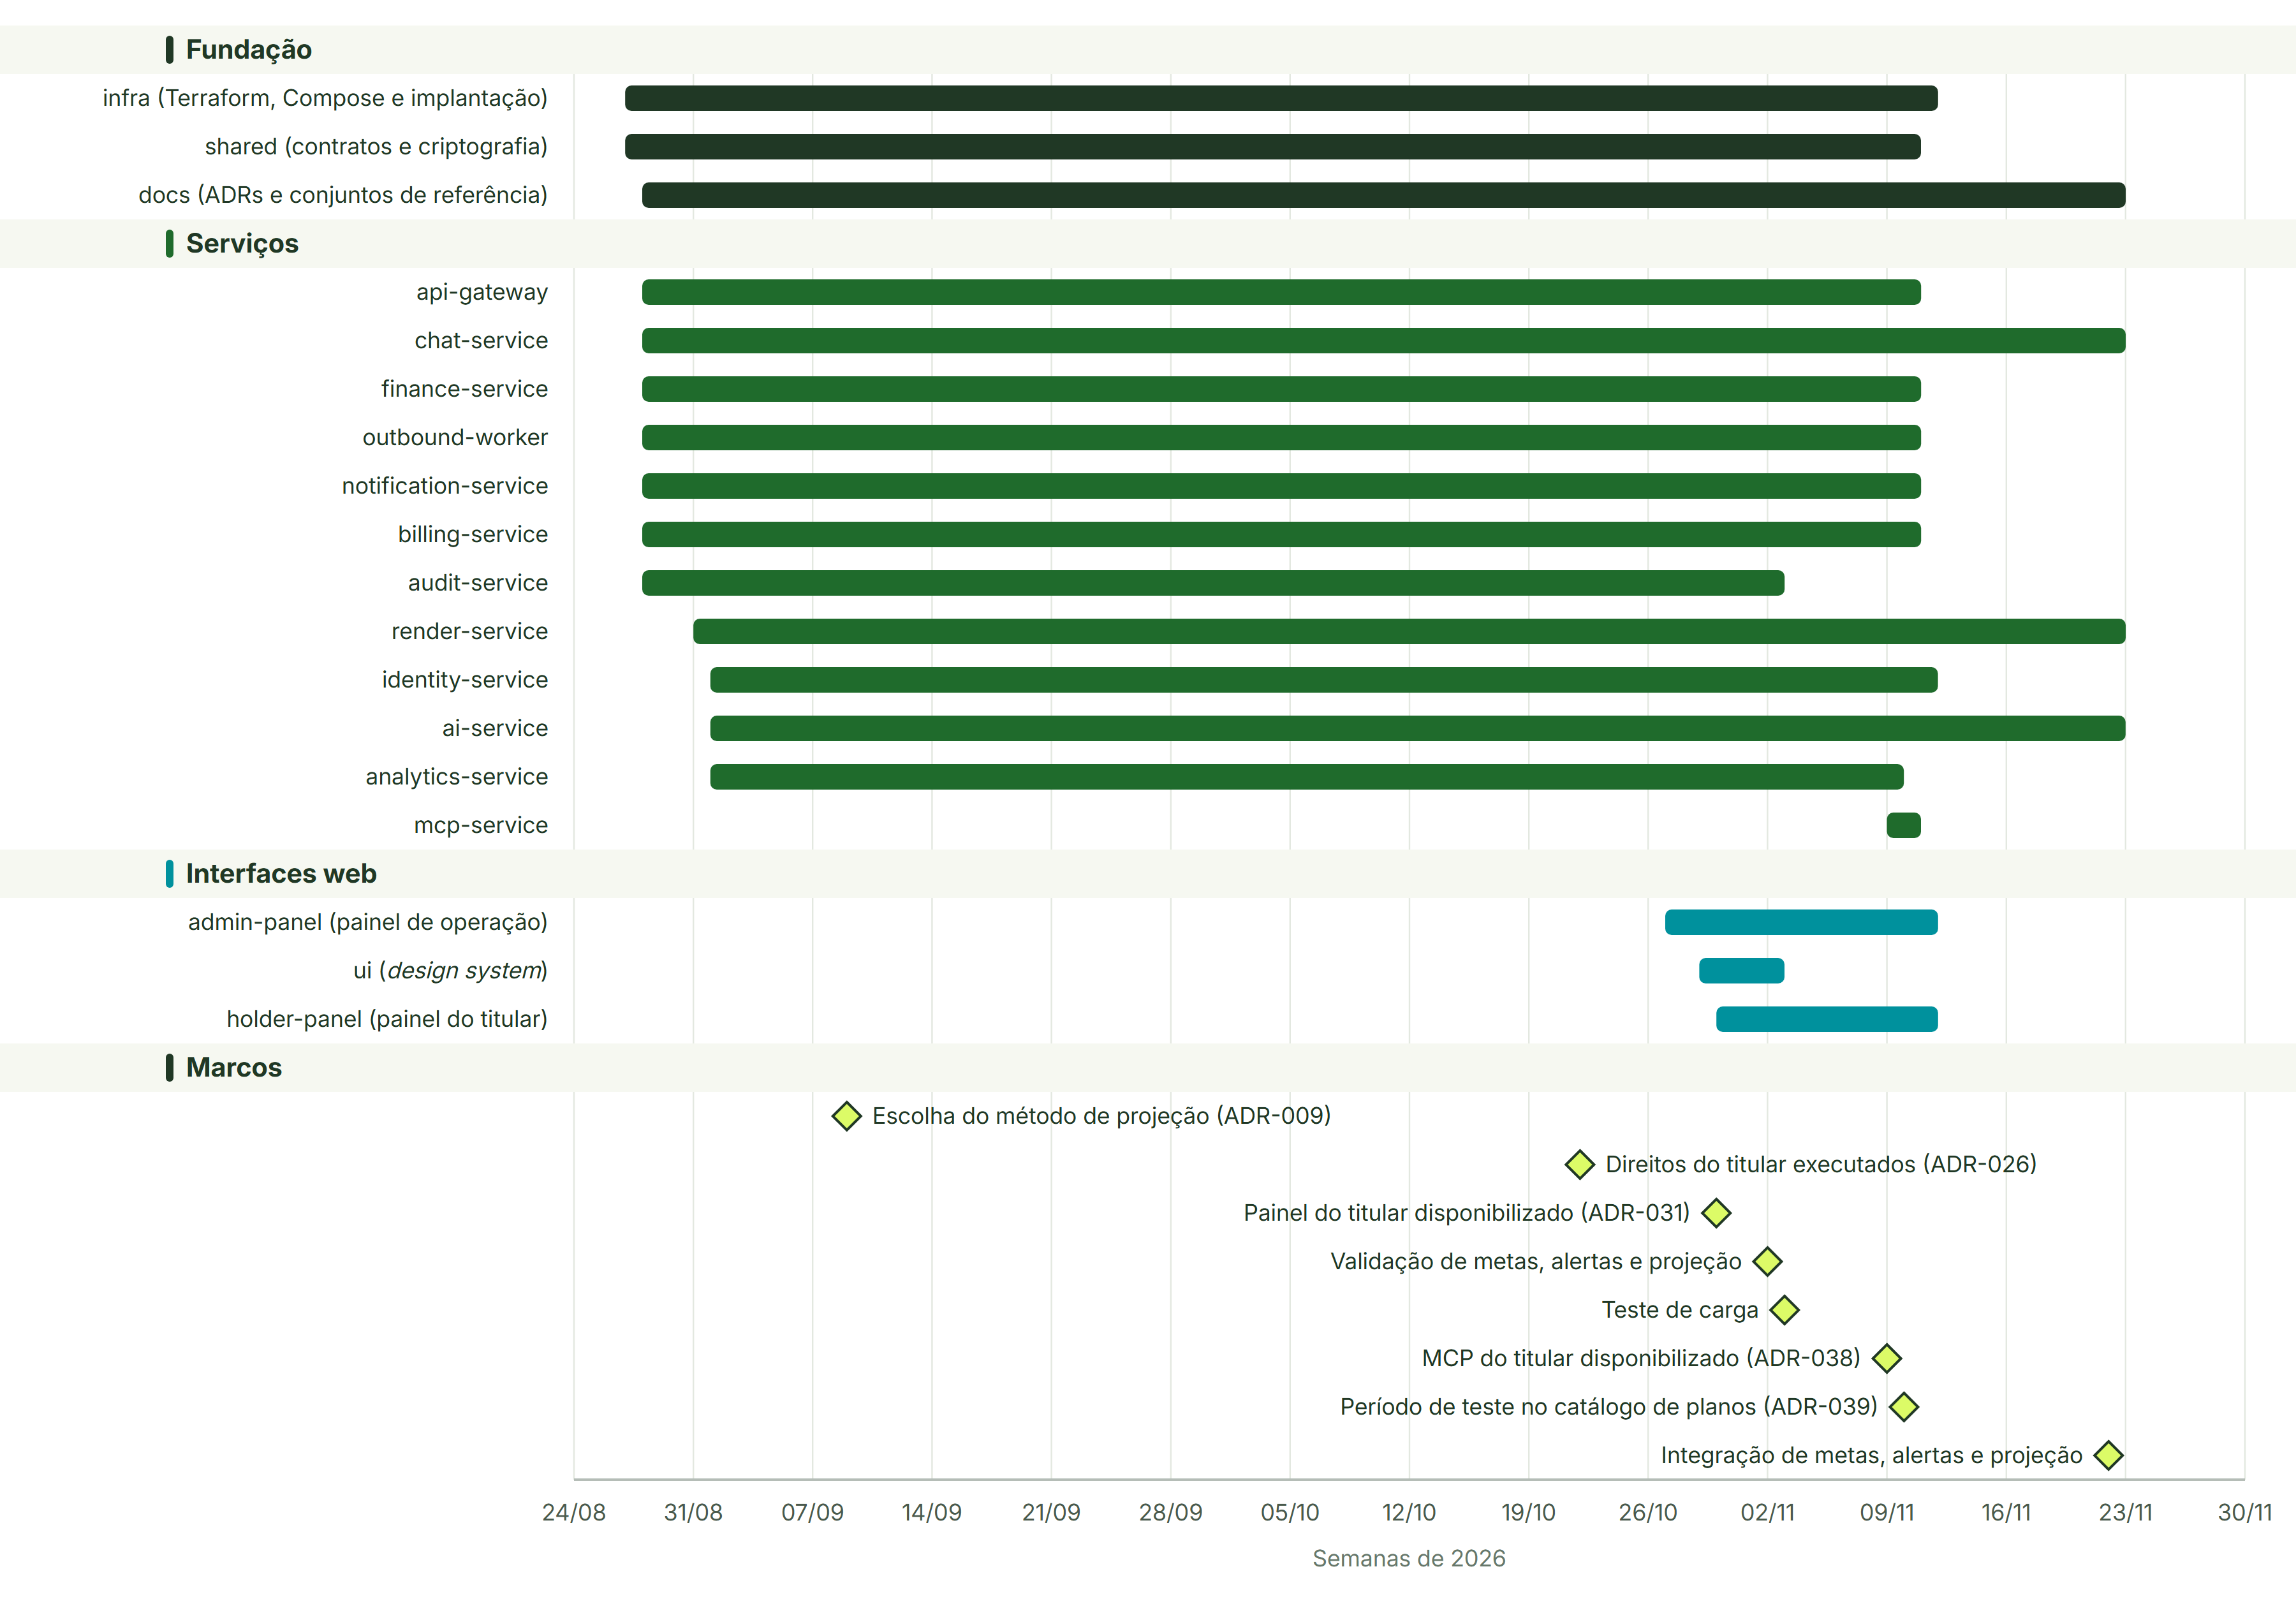
\includegraphics[width=1\textwidth]{images/cronograma_desenvolvimento.png}
    \authorssource
\end{figure}

\section{Matriz SWOT}

A Matriz SWOT constitui uma ferramenta de apoio à análise estratégica que reúne, em uma avaliação global, as forças e as fraquezas internas de um empreendimento, bem como as oportunidades e as ameaças do ambiente externo (KOTLER; KELLER, 2012). Nesse sentido, a Figura~\ref{fig:swot} apresenta as forças, fraquezas, oportunidades e ameaças identificadas para o EIGAM.

\begin{figure}[H]
    \centering
    \caption{Matriz SWOT}
    \label{fig:swot}
    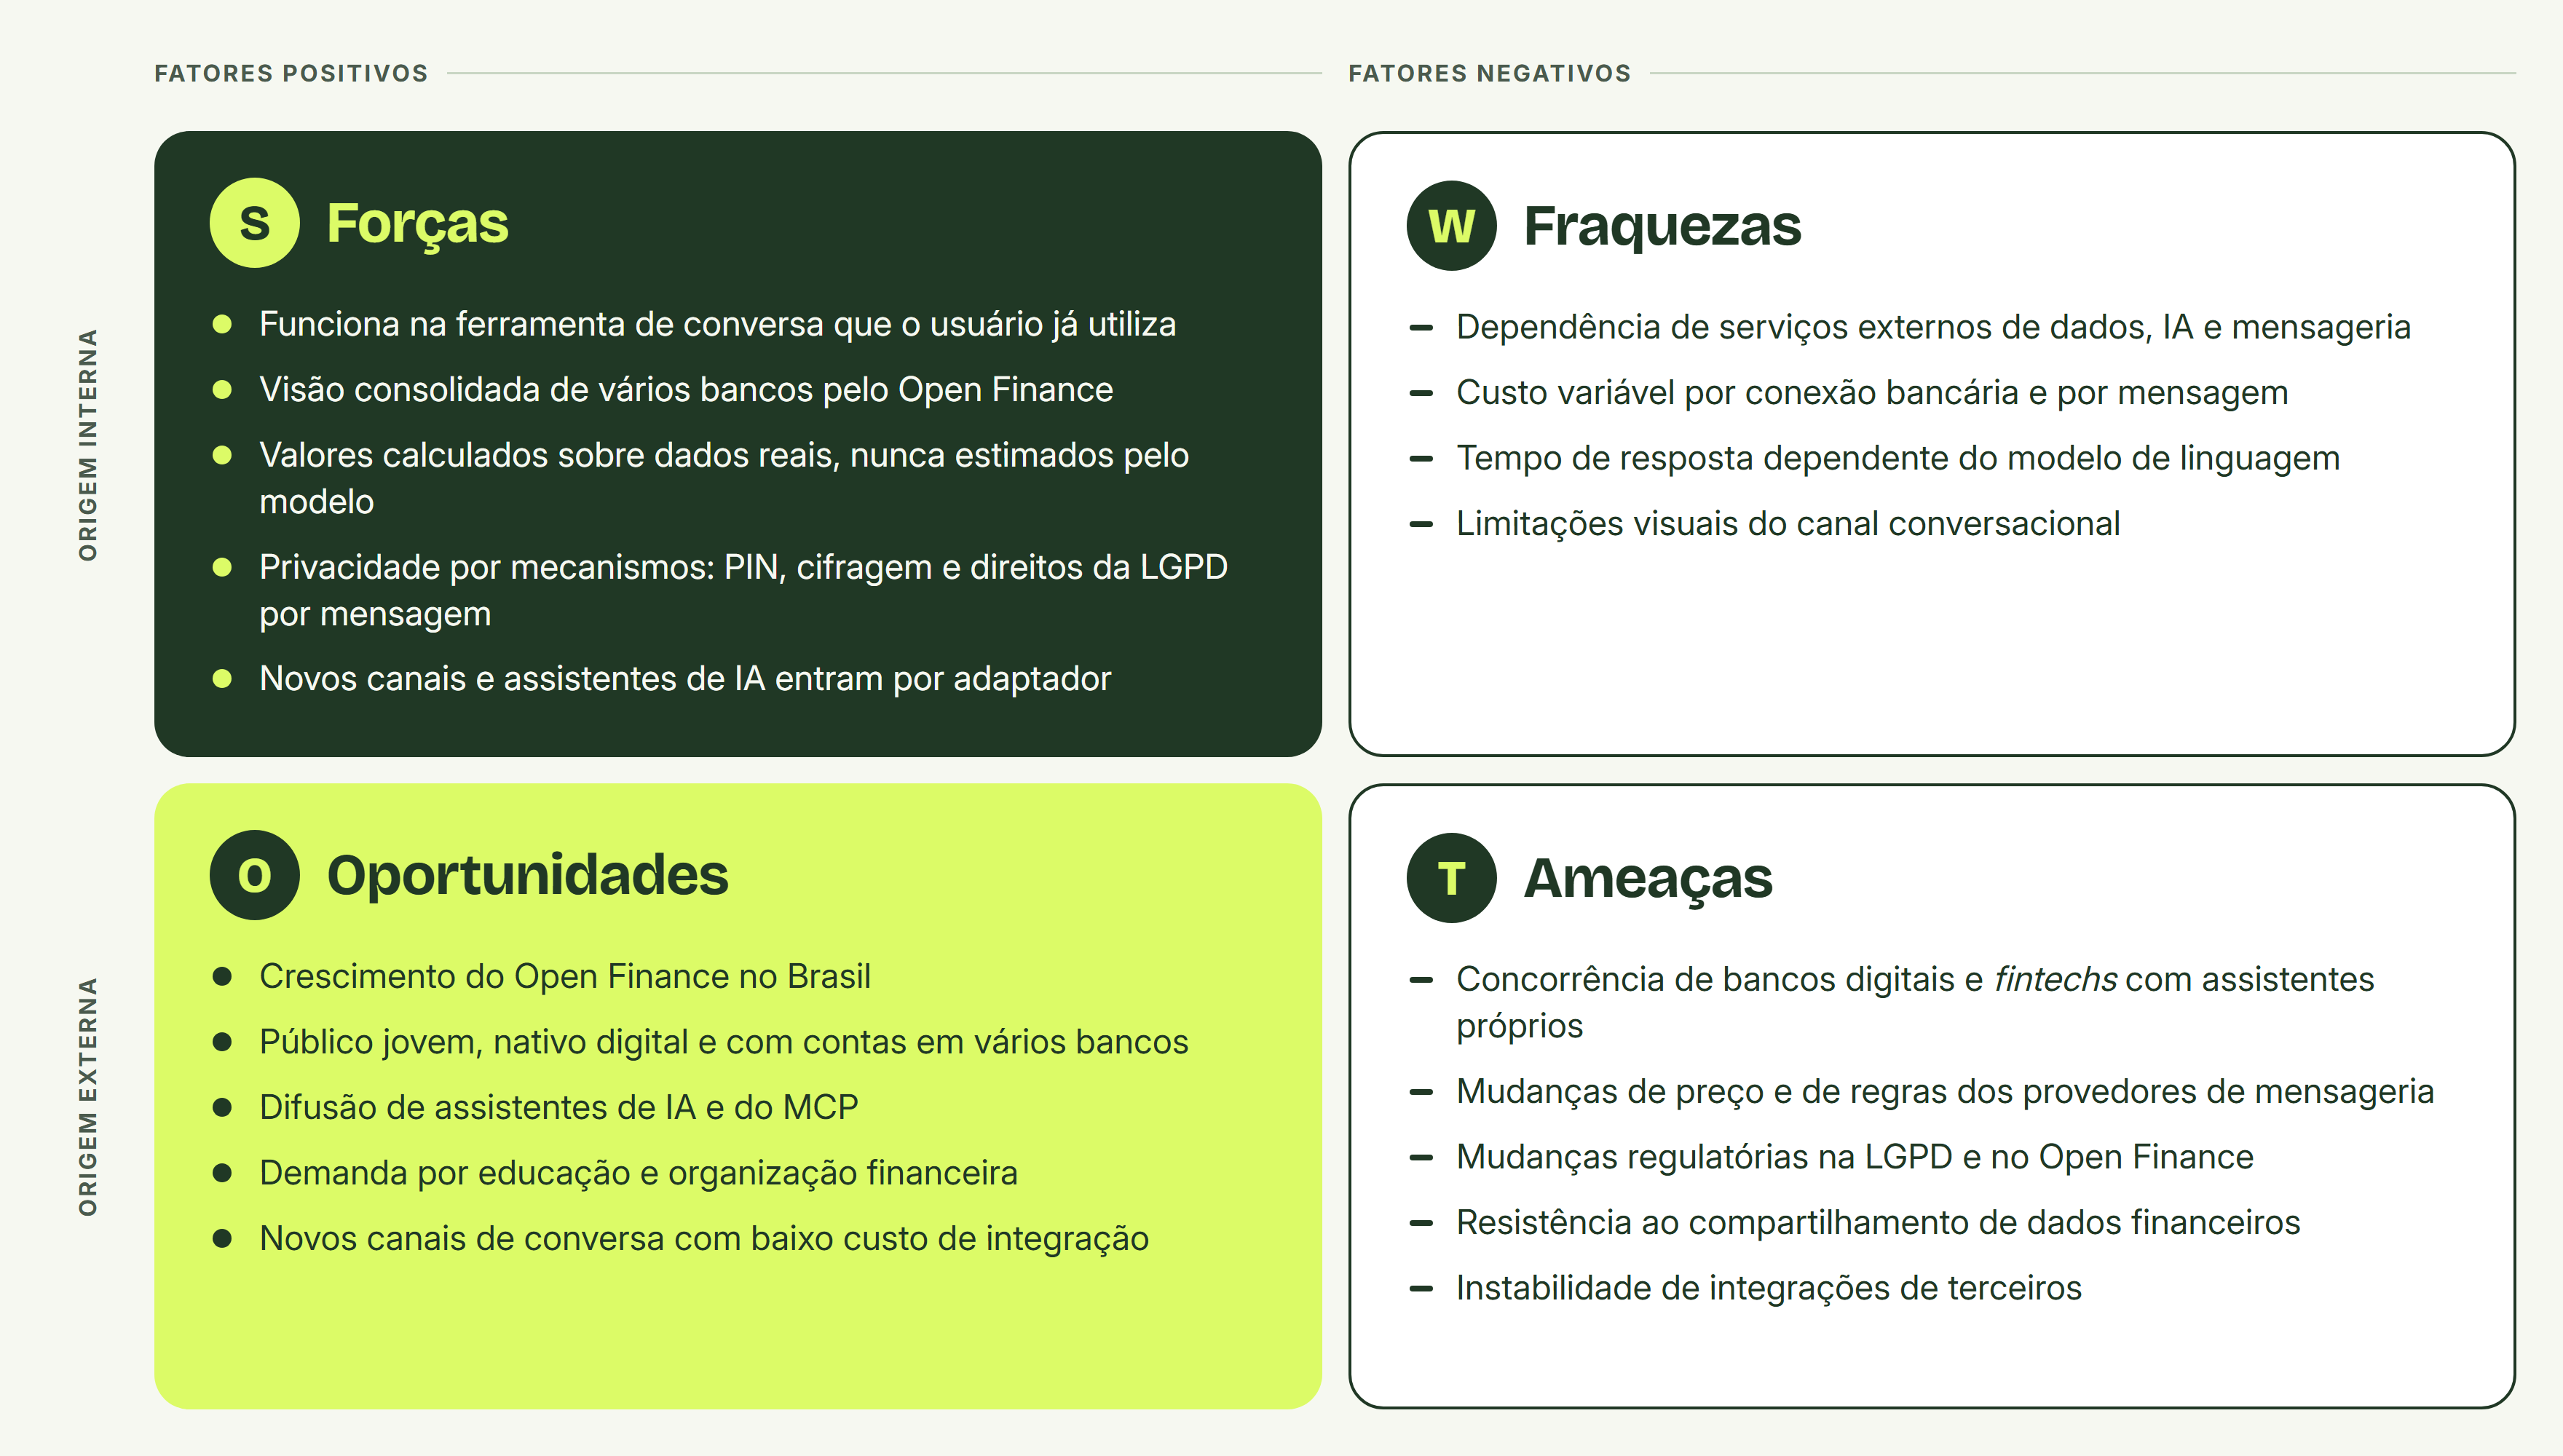
\includegraphics[width=1\textwidth]{images/swot.png}
    \sourcenote{\textbf{Fonte:} Elaborado pelos autores (\workYear), com base em Kotler e Keller (2012).}
\end{figure}

A leitura da matriz mostra que as forças do EIGAM vêm de decisões de arquitetura e de privacidade: o funcionamento na ferramenta de conversa que o usuário já utiliza, a visão consolidada de vários bancos, os valores calculados sobre dados reais e a proteção por PIN, pela cifragem e pelos direitos da LGPD exercidos por mensagem. As fraquezas concentram-se na dependência de serviços externos e nos custos variáveis por conexão bancária e por mensagem, que o período de teste e o plano Pro ajudam a controlar. No ambiente externo, o crescimento do Open Finance e a difusão de assistentes de IA favorecem a proposta, enquanto a concorrência de bancos digitais e \textit{fintechs} é a principal ameaça, e as mudanças de preço e de regras dos provedores de mensageria reforçam o valor da arquitetura desacoplada do canal.
